\section{External documents: an important counterexample}
\label{sec:external}
To test a different input form, we extend the earlier raw-document/wiki experiment with 132 actual Opus 5.5 calls: six contexts on 22 visible development questions from one externally authored fictional company. Its 118 source pages are MIT-licensed material from GBrain's evaluation repository. The two wikis were compiled previously by an actual query-blind GPT process, without questions or labels. We replay the exact saved contexts with Opus adaptive/high and an 8,192-token output allowance; no wiki is rewritten after seeing these answers.

\begin{figure}[t]
\centering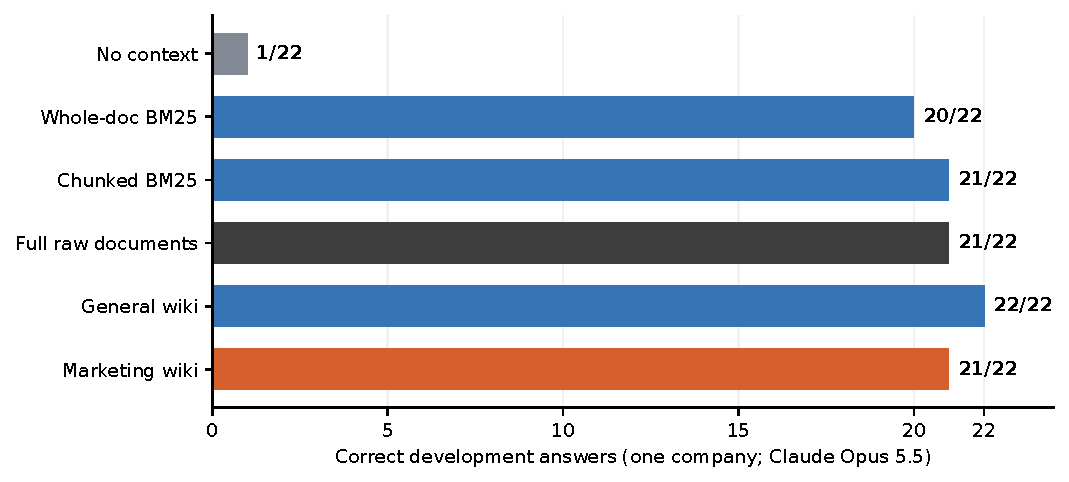
\includegraphics[width=\linewidth]{figures/challenge/external.pdf}
\caption{Exploratory raw-document/wiki QA with Opus: the general wiki outperforms the marketing wiki by one answer. This is one company with 22 development questions, not 22 independent companies or a recommendation-utility benchmark. No company-population uncertainty is inferred.}
\label{fig:external}
\end{figure}

\begin{table}[t]
\centering\small\begin{tabular}{lrrr}
\toprule
Context & Correct / 22 & Excluding ambiguous item / 21 & Reader USD \\
\midrule
No context & 1 & 1 & 0.10 \\
Whole-doc BM25 & 20 & 20 & 1.04 \\
Chunked BM25 & 21 & 21 & 1.06 \\
Full raw documents & 21 & 21 & 10.74 \\
General wiki & 22 & 21 & 2.60 \\
Marketing wiki & 21 & 20 & 2.45 \\
\bottomrule
\end{tabular}

\caption{Original upstream labels and a separately disclosed sensitivity excluding the known ambiguous July ownership question. Every original score remains retained. Reader USD excludes the earlier shared wiki compilation. Valid citation IDs do not establish semantic entailment.}
\label{tab:external}
\end{table}

The general wiki answers 22/22 correctly; the marketing wiki answers 21/22. Whole-document BM25 scores 20/22, while chunked retrieval and full raw context score 21/22. All calls complete. Excluding the known ambiguous item leaves general wiki, full raw and chunked retrieval at 21/21, but the marketing wiki at 20/21 (Table~\ref{tab:external}). This is conditional evidence against universal specialization superiority, not an estimate of a one-answer market advantage.

We review all five non-no-context errors. The marketing-wiki error misidentifies ``Dana's freight account'' in a dated handoff: the source explicitly links the phrase to Quarrendon. Both compiled wikis omit that literal phrase but retain ownership dates; Opus resolves them correctly with the general wiki and incorrectly with the marketing wiki. This is a context/reader interaction, not proof that specialization deleted the required date facts. Three raw-context errors concern the upstream July ownership ambiguity. Whole-document BM25 also misses an oversized contract clause that chunking recovers. These cases explain why compilation, packing and reference-label sensitivity need separate scrutiny. Earlier GPT/Sonnet outcomes remain archived, with different effort settings; they are not a controlled model-only comparison with this extension.
